\chapter{Channel segregation in mono-grains}

\comment{this appendix is temporary, it may be deleted later}

All CAFE simulations were performed considering a normal classic heterogeneous nucleation at 
the surface of the mould where the metal is cooled down. However, as the number of grains is
not negligible, the subsequent fluid-structure interaction between dendrites, simply represented by an isotropic permeability 
and the interdendritic flow cannot be easily interpreted. Therefore, one may consider simpler solidification cases 
like a mono-grain growth. This ideal situation is not always experimentally viable: either the mould surface is not 
perfectly smooth, and therefore nucleation can be triggered by a wetting mechanism, or the metal contains a certain level of impurity
which can trigger nucleation heterogeneously in the liquid bulk. 
Regardless of this experimental limitation, this type of simulations allows simpler understanding as the grain growth is not 
disturbed by another neighbouring grain, it grows while exclusively interacting with the liquid phase.

%----------------------------
\ifthenelse{\boolean{enable_animations}}%
  {% then
    %-------
    \begin{figure}[htbp]
    \centering %
    \begin{animateinline}{6}%
      %\multiframe{nb_frames}{i=start_nb+inc_nb}{%
       \multiframe{108}{i=25+1}{%     
        \includegraphics[height=6cm]{Chapter4/Graphics/freckle_cafe/anim_monograin_upright/img\zeropad{1234}{\i}.png}%
        \hspace{1mm}%
          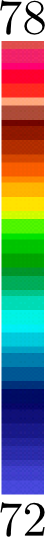
\includegraphics[height=6cm]{Chapter4/Graphics/freckle_cafe/cafe_VG_colorbar_annot.png}%
        \hspace{1mm}%      
          \includegraphics[height=6cm]{Chapter4/Graphics/freckle_cafe/anim_monograin_tilted/img\zeropad{1234}{\i}.png}%
      }%
    \end{animateinline}%
    \caption{Animations of mono-grain solidification showing the average composition in gallium predicted by the CAFE approach. 
    Two orientation scenarios are considered where a) the grain is upright with a Euler angle of \orient{90}{0}{0} 
    or b) the grain is tilted with a Euler angle of \orient{90}{30}{0}.}
    %-------    
    \label{fig:animate_monograin}
    \end{figure}
  }
  {% else 
  \begin{figure}[htbp]
  %\centering
   %------------
      \begin{subfigure}[t]{0.35\textwidth}
        %\centering
      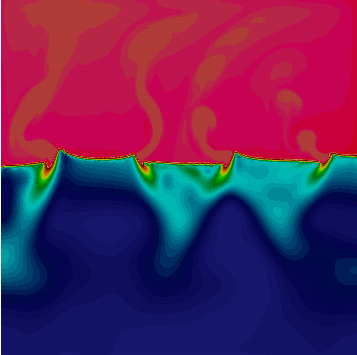
\includegraphics[height=6cm]{Chapter4/Graphics/freckle_cafe/anim_monograin_upright/img0133.png}%
      \caption{}
        \end{subfigure}
        %-----
        \hspace{10mm}
        \begin{subfigure}[t]{0.15\textwidth}
        \centering
      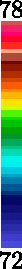
\includegraphics[height=6cm]{Chapter4/Graphics/freckle_cafe/cafe_VG_colorbar_annot.pdf}%
      %\caption{}
        \end{subfigure}
        %-----
        %\hspace{1mm}
        \begin{subfigure}[t]{0.35\textwidth}
        \centering
      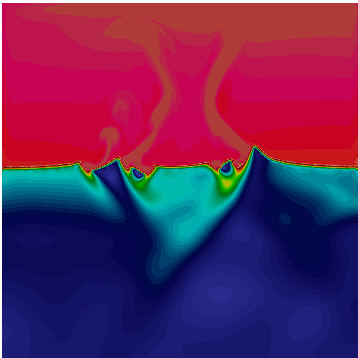
\includegraphics[height=6cm]{Chapter4/Graphics/freckle_cafe/anim_monograin_tilted/img0133.png}%
      \caption{}
        \end{subfigure}
        %-----
          \caption{Snapshots of mono-grain solidification showing the average composition in gallium predicted by the CAFE approach. 
      Two orientation scenarios are considered where a) the grain is upright with a Euler angle of \orient{90}{0}{0} 
      or b) the grain is tilted with a Euler angle of \orient{90}{30}{0} (check animation in the PDF file).}
      %-------
      \label{fig:animate_monograin}
      \end{figure}
  }
%--------------
%===================================== ANIMATION FIGURE with \animage =====================================
% \begin{figure}[htbp]
% \centering
  %------------
  % \begin{subfigure}{0.45\textwidth}
  % \centering
  % \animage{height=6cm}{6}{Chapter4/Graphics/freckle_cafe/anim_monograin_upright/img0}{030}{133}{.png} % 0000 to 0139
  % \caption{}
    % \label{fig:mono_upright}
  % \end{subfigure}  
  %------------
  % \hfill %\hspace{1mm}  
   % \begin{subfigure}{0.05\textwidth}
  % \centering
  % 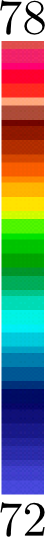
\includegraphics[height=6cm]{Chapter4/Graphics/freckle_cafe/cafe_VG_colorbar_annot.png}
  % \caption{}
    % \label{} % Do not delete or comment this line to preserve alignment
  % \end{subfigure}
  % \hfill %\hspace{1mm}  
  %------------
  % \begin{subfigure}{0.45\textwidth}
    % \centering
    % \animage{height=6cm}{6}{Chapter4/Graphics/freckle_cafe/anim_monograin_tilted/img0}{030}{133}{.png} % 0000 to 0133
  % \caption{}
    % \label{fig:mono_tilted}
  % \end{subfigure}
%-------
% \caption{Animations of mono-grain solidification showing the average composition in gallium predicted by the CAFE approach. 
% Two orientation scenarios are considered where a) the grain is upright with a Euler angle of \orient{90}{0}{0} 
% or b) the grain is tilted with a Euler angle of \orient{90}{30}{0}.}
% \label{fig:animate_monograin}
% \end{figure}
%===================================== ANIMATION FIGURE =====================================